\subsection{Sinking hydrated cylinder}\label{sec:quinquis}
This experiment is performed as explained in \citet{Quinquis2014} and simulates the sinking of a cold, hydrated cylinder into a warm, dry mantle. The domain
is square with $L_x=L_y=$ \SI{300}{\km}, a grid resolution of $300\times300$ elements and 25 markers per element. The sinking cylinder is located at $x=$
\SI{150}{\km} and $y=$ \SI{170}{\km} with a radius of \SI{20}{\km} and has $\rho_c=$ \SI{3250}{\kg\per\cubic\m}, $\eta_c=$ \SI{e23}{\pascal\s}, a thermal
conductivity $k_c=$ \SI{4.5}{\watt\per\m\per\kelvin},a specific heat $C_{p_c}=$ \SI{1250}{\joule\per\kg\per\kelvin}; the surrounding mantle has $\rho_m=$
\SI{3200}{\kg\per\cubic\m}, $\eta_m=$ \SI{e20}{\pascal\s}, a thermal conductivity $k_m=$ \SI{105}{\watt\per\m\per\kelvin} and specific heat $C_{p_m}=$
\SI{1250}{\joule\per\kg\per\kelvin}; a 58 km-thick lithosphere overlies the mantle and has $\rho_l=$ \SI{3200}{\kg\per\cubic\m}, $\eta_l=$ \SI{e23}{\pascal\s},
a thermal conductivity $k_l=$ \SI{4.5}{\watt\per\m\per\kelvin}, specific heat $C_{p_l}=$ \SI{750}{\joule\per\kg\per\kelvin} and a thermal diffusivity of
\SI{e-6}{\square\m\per\s}. Velocity boundary conditions are set to free slip on all sides of the domain. Temperature increase linearly in the lithosphere,
from 0° to 1300°C, and in the mantle, from 1300° to 1360.5°C. The initial temperature of the cylinder is fixed to 400°C. Throughout the evolution, temperature
is fixed to 0° and 1360.5°C at the top and bottom of the domain, respectively. The initial bound water content is imposed at 2 wt.\% in the cylinder and at
0 wt.\% in both the mantle and the lithosphere. The maximum amount of water in the mantle is fixed to 0.2 wt.\%, while maximum water content in the cylinder
and in the lithosphere is function of pressure and temperature and is calculated using a serpentinized harzburgite with Perple\_X, as in \citet{Quinquis2014}.

As shown in \citet{Quinquis2014}, the model is characterised by a progressive dehydration in the external portion of the cylinder, due to the increase of
temperature, with a consequent vertical migration of free water that hydrates the mantle above the cylinder, up to the lithosphere. The distribution of
bound and free water during the evolution of the experiment is shown in Fig. \ref{fig:quinquis} (left and right columns, respectively). 
All data can be found at \url{https://github.com/aleregorda/Benchmarks/tree/main/Hydration}.

\begin{figure}
\centering
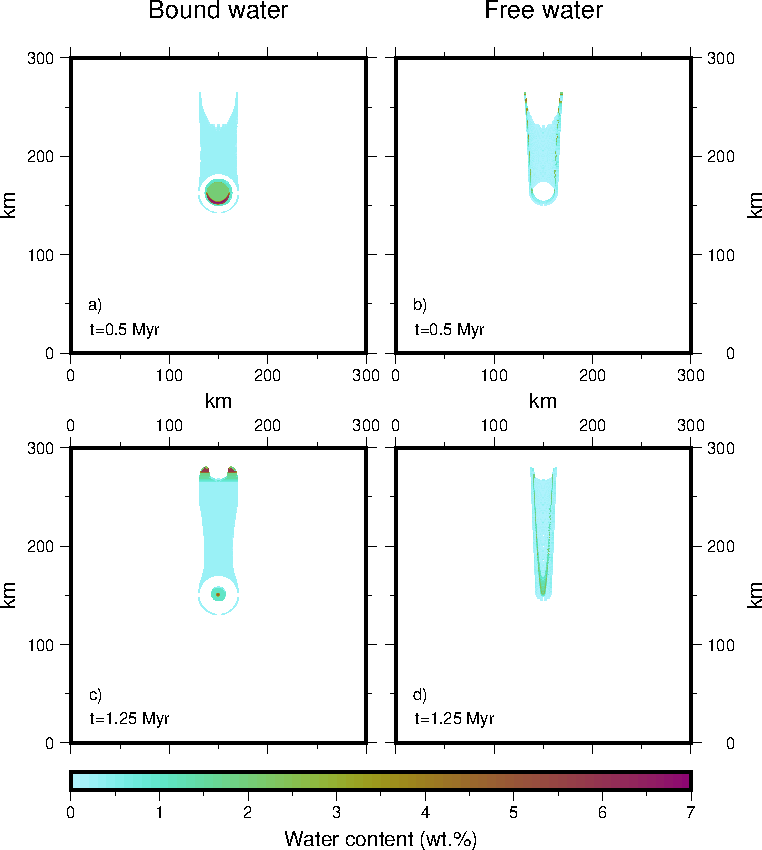
\includegraphics[width=400px]{./Figures/Hydration.pdf}
\caption{Distribution of bound and free water (left and right columns, respectively) at $t=0.5$ and $t=$ \SI{1.25}{\mega\year} (first and second rows,
respectively) for the sinking hydrated cylinder experiment. Only markers with bound or free water not equal to 0 are plotted.}
\label{fig:quinquis}
\end{figure}